\subsection{Coverage vs.\ Physical Realism (dt-fixed=30s)}
We evaluate under a strict dt-fixed ($\Delta t=30$s) protocol. To characterize the coverage--realism tension in non-residual diffusion variants, we first report results on a diagnostic set of 320 sampled test conditions (Table~\ref{tab:phaseb_quick}). The deterministic prior (L2 regression) is evaluated with $K=1$, while diffusion-based generators use $K=20$ samples per condition.

\begin{table}[t]
  \centering
  \small
  \begin{tabular}{lrrrrrrr}
    \toprule
    Model & $K$ & ADE$_{\text{mean}}$ & ADE$_{\text{best}}$ & FDE$_{\text{mean}}$ & FDE$_{\text{best}}$ & MSD$_{10}$ & Rog \\
    \midrule
    Deterministic prior (L2) & 1  & 5.467 & 5.467 & 8.855  & 8.855  & 304.099 & 5.494 \\
    Diffusion                & 20 & 6.741 & 2.836 & 11.636 & 3.950  & 100.948 & 3.056 \\
    Physics (nav conditioning) & 20 & 6.744 & 2.510 & 11.644 & 3.419  & 116.869 & 3.435 \\
    \bottomrule
  \end{tabular}
  \caption{Diagnostic results on 320 sampled test conditions under dt-fixed=30s. MSD$_{10}$ corresponds to a lag of $10\Delta t=300$s. Ground-truth macro references on the same conditions are GT\_Rog=5.247 and GT\_MSD$_{10}$=349.740.}
  \label{tab:phaseb_quick}
\end{table}

\paragraph{Micro-level errors and coverage.}
As expected, the deterministic prior achieves the lowest mean errors (Table~\ref{tab:phaseb_quick}). Diffusion improves multi-modality: best-of-$K$ (oracle; minimum error over $K$ samples) errors are substantially lower, indicating stronger coverage. Navigation field conditioning further improves the oracle upper bound (Physics vs.\ Diffusion in ADE$_\text{best}$ and FDE$_\text{best}$).

\paragraph{Macro-level physical realism: shrinkage in pure diffusion.}
Despite strong best-of-$K$, pure diffusion under-estimates macroscopic motion (Table~\ref{tab:phaseb_quick}). Navigation field conditioning improves these statistics modestly but does not eliminate the gap. Figure~\ref{fig:phaseb_quant} visualizes the same pattern via micro summaries and MSD curves.

\begin{figure}[t]
  \centering
  \begin{subfigure}[t]{\linewidth}
    \centering
    
\includegraphics[width=0.98\linewidth]{figures/fig1_micro_metrics.png}
    \caption{Micro-level metrics (mean/std and best-of-$K$ where applicable).}
    \label{fig:phaseb_micro}
  \end{subfigure}

  \vspace{0.4em}
  \begin{subfigure}[t]{\linewidth}
    \centering
    
\includegraphics[width=0.90\linewidth]{figures/fig2_msd_curve.png}
    \caption{MSD curves (Pred vs.\ GT) under dt-fixed=30s.}
    \label{fig:phaseb_msd}
  \end{subfigure}
  \caption{Quantitative evidence under dt-fixed=30s: diffusion improves best-of-$K$ coverage but exhibits macroscopic shrinkage in MSD/Rog.}
  \label{fig:phaseb_quant}
\end{figure}

\subsection{Main Result: Residual Diffusion Mitigates Shrinkage}
To separate macroscopic motion scale from stochastic variation, we apply residual diffusion (Eq.~\ref{eq:residual_decomp}), using the frozen deterministic prior and learning diffusion residuals. Table~\ref{tab:residual_test} reports a leakage-free evaluation on a larger set of 51,200 test conditions ($K=10$): residual diffusion restores macroscopic scale while retaining strong best-of-$K$ behavior. Residual Physics (residual diffusion with navigation field conditioning) further improves best-of-$K$, but its macroscopic statistics remain slightly conservative.
Here, Speed Ratio is defined as $\mathbb{E}[\|\mathbf{v}\|_2]_{\mathrm{pred}}/\mathbb{E}[\|\mathbf{v}\|_2]_{\mathrm{gt}}$, where $\mathbb{E}[\cdot]$ denotes the mean over future timesteps and evaluated conditions. Rog Ratio is $\mathrm{Rog}_{\mathrm{pred}}/\mathrm{Rog}_{\mathrm{gt}}$, and MSD$_{10}$ Ratio is $\mathrm{MSD}_{10,\mathrm{pred}}/\mathrm{MSD}_{10,\mathrm{gt}}$ computed on the same conditions.

\begin{table}[t]
  \centering
  \small
  \begin{tabular}{lrrrrr}
    \toprule
    Model & $K$ & Speed Ratio & Rog Ratio & MSD$_{10}$ Ratio & ADE$_{\text{best}}$ \\
    \midrule
    Residual Diffusion   & 10 & 1.016 & 1.004 & 0.935 & 3.656 \\
    Residual Physics (nav conditioning) & 10 & 0.951 & 0.945 & 0.864 & 2.709 \\
    \bottomrule
  \end{tabular}
  \caption{Residual variants on the test split (51,200 conditions; $K=10$). Ratios are computed against ground-truth statistics on the same evaluated conditions under the same protocol.}
  \label{tab:residual_test}
\end{table}

\paragraph{Qualitative geographic-space visualization (Scheme B).}
To connect model behavior to urban spatial structure, we visualize saved evaluation samples (N=80 conditions) in geographic space via a linear bbox projection (without road-level map matching). Figure~\ref{fig:residual_geo_overlay} compares the deterministic prior with residual diffusion. The panel title ``Diffusion'' denotes the diffusion-based generator; in this figure it corresponds to the residual diffusion variant.

\begin{figure}[t]
  \centering
  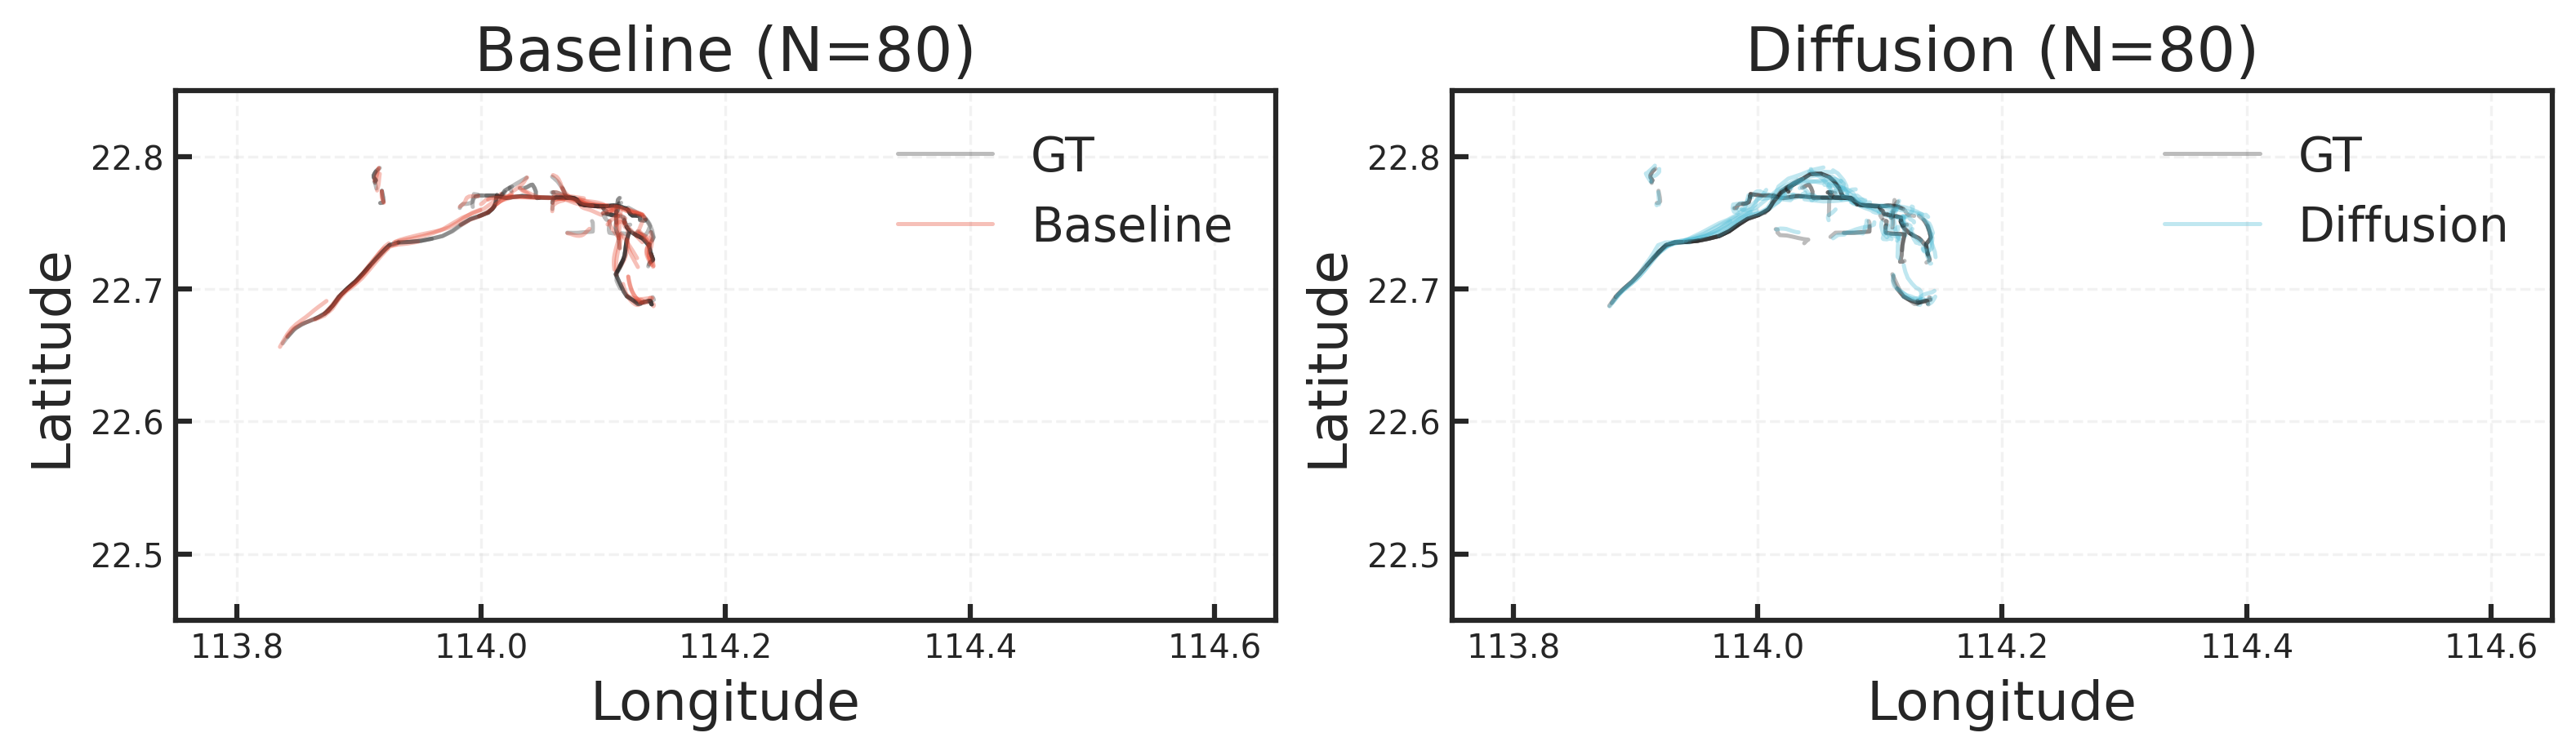
\includegraphics[width=0.95\linewidth]{figures/fig_geo_traj_overlay_v11.png}
  \caption{Geographic-space visualization (trajectory overlays). Left: deterministic prior (L2 regression). Right: residual diffusion (v1.1).}
  \label{fig:residual_geo_overlay}
\end{figure}

\subsection{CFG as an Inference-Time Micro--Macro Knob (Shenzhen Geo-Scale)}
The residual formulation addresses the \emph{structural} shrinkage issue by anchoring macroscopic scale to a deterministic prior. Building on this foundation, we introduce \emph{classifier-free guidance} (CFG) at inference time to control how strongly the generator is attracted to the known destination. This yields an interpretable trade-off: a moderate CFG emphasizes micro-level precision (best-of-$K$), while a stronger CFG emphasizes macro-level validity (MSD/Rog) by more aggressively enforcing OD intent.

\paragraph{Protocolized settings (avoid hyperparameter swamp).}
Following the PI review, we report two pre-registered CFG settings rather than an open-ended sweep:
\textbf{cfg=2} is \emph{micro-optimal} under a macro validity gate, while \textbf{cfg=3} demonstrates that the same trained model can be tuned toward \emph{macro-validity} at the cost of micro-precision.
Figure~\ref{fig:cfg_pareto} summarizes this curve on validation data.

\begin{figure}[t]
  \centering
  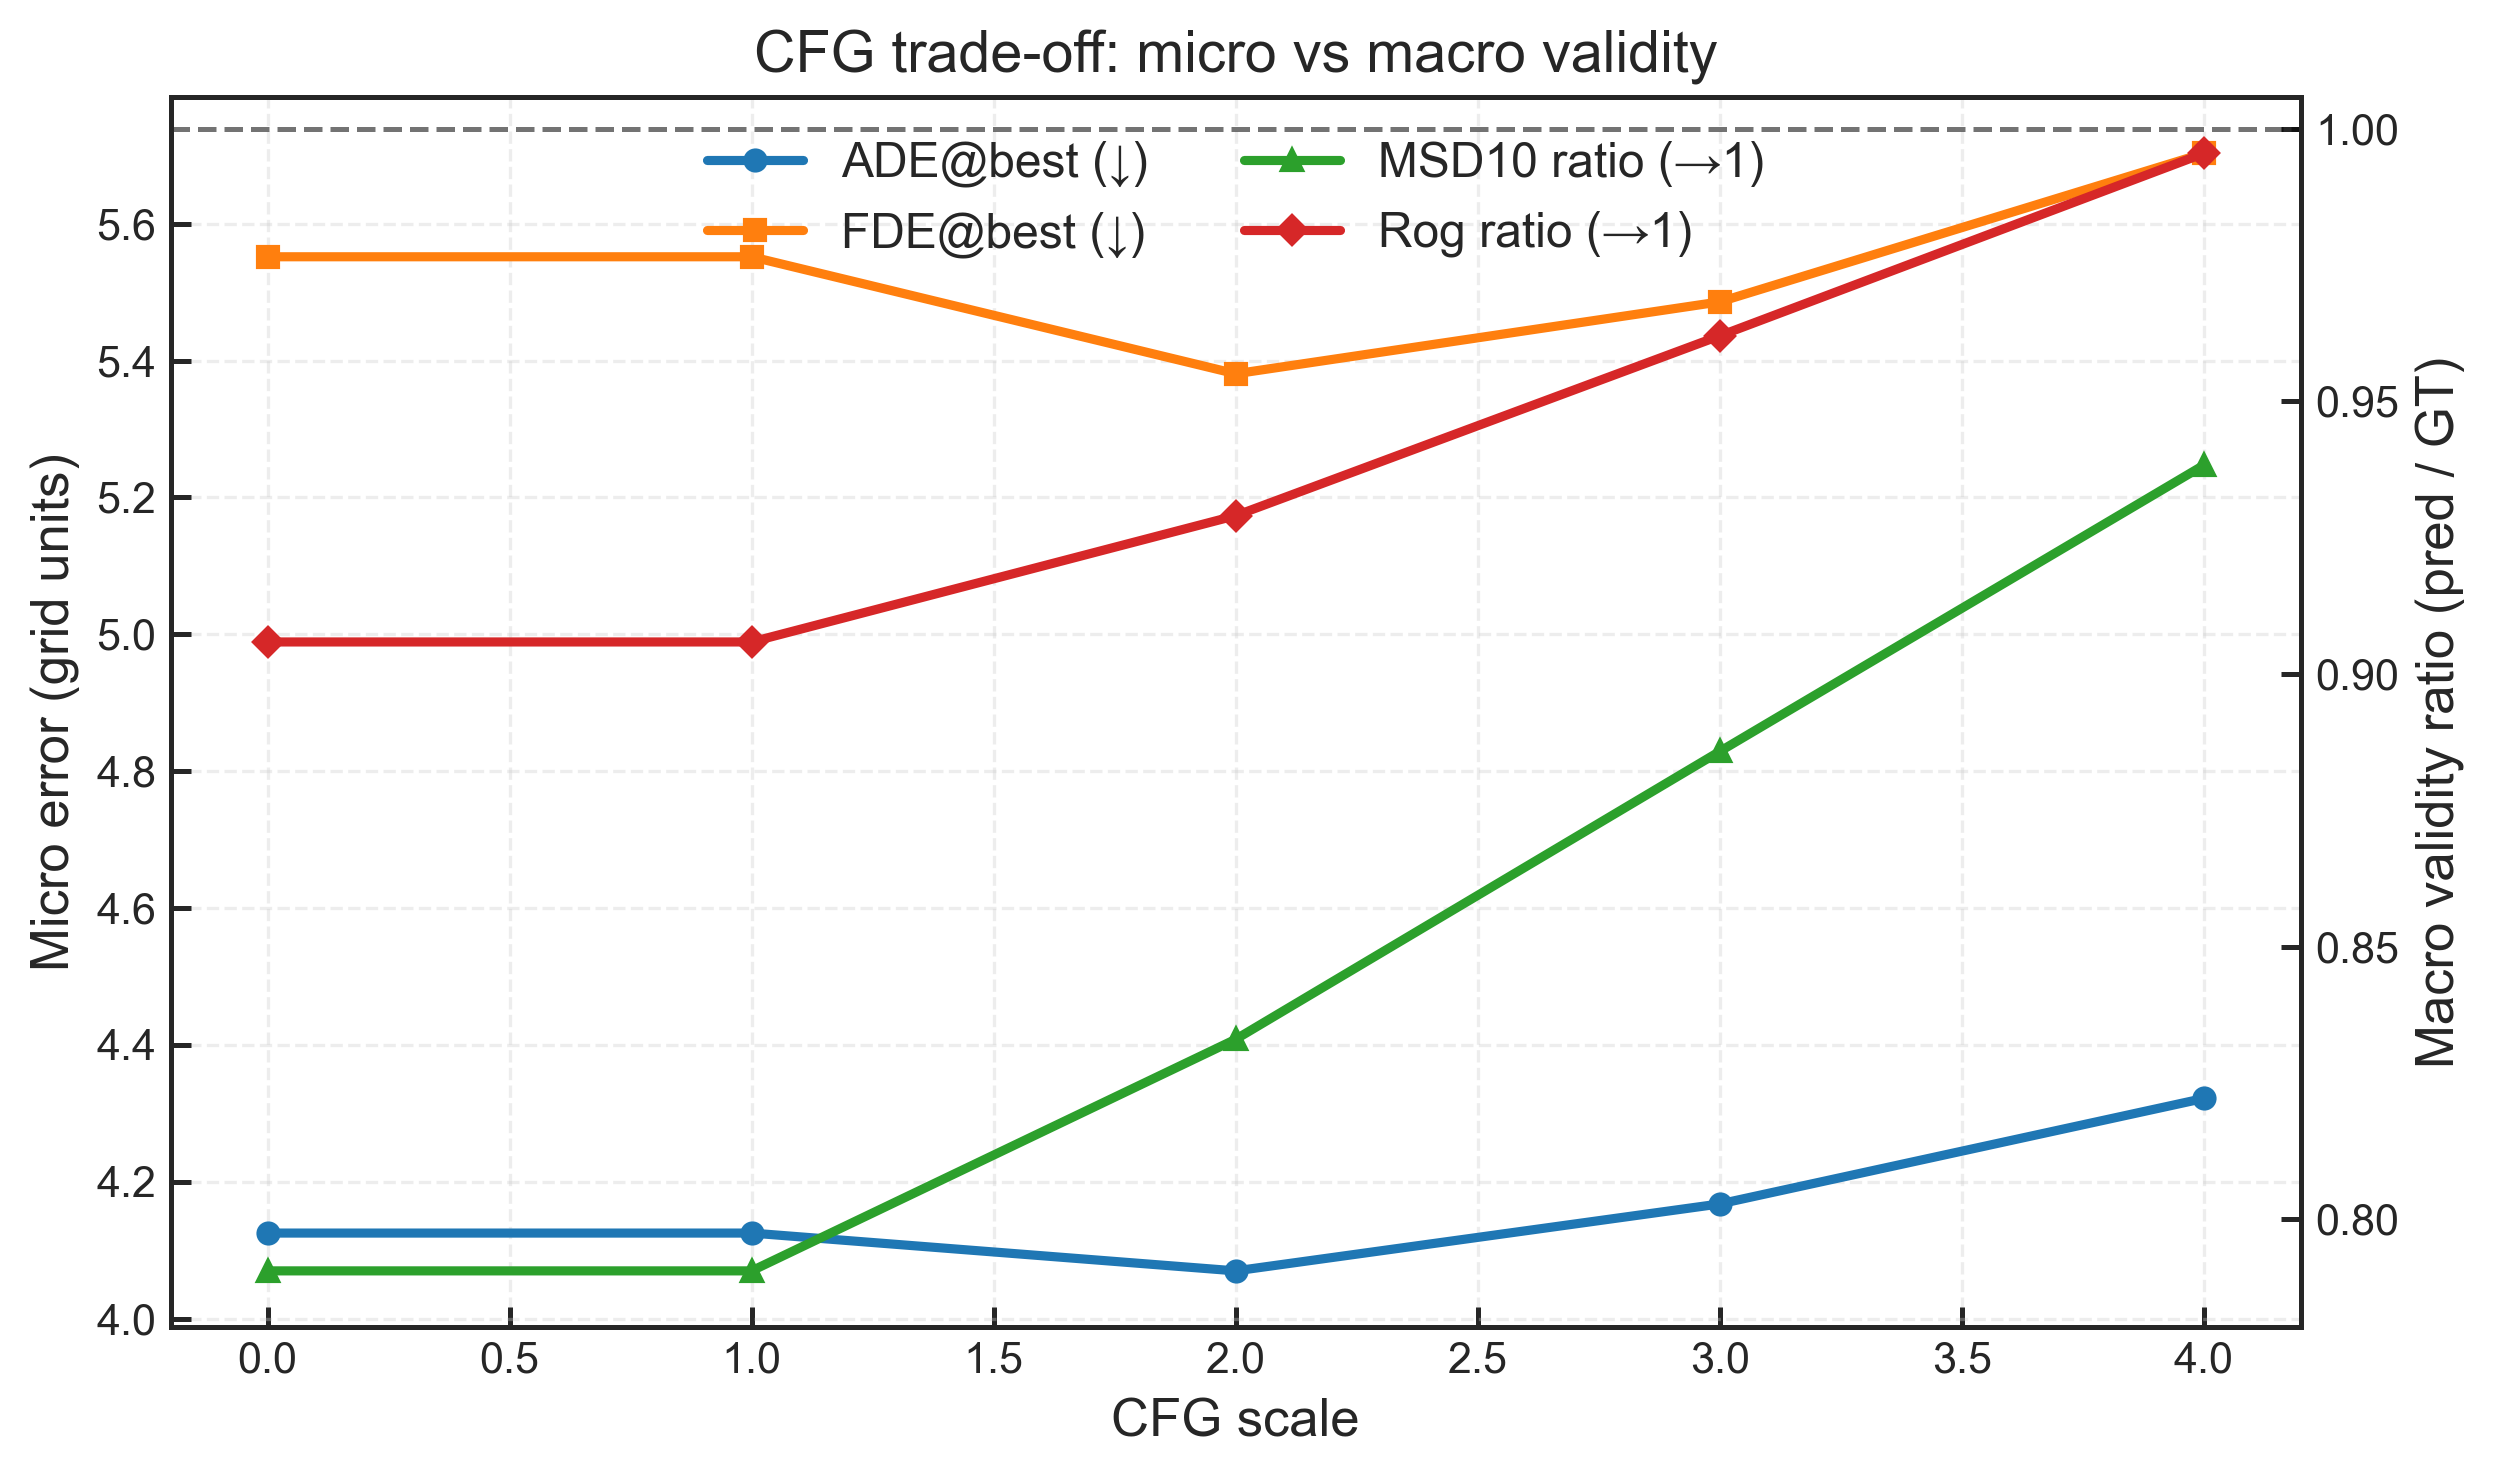
\includegraphics[width=0.92\linewidth]{figures/stage_cfg/fig_cfg_pareto.png}
  \caption{CFG trade-off curve on validation: micro errors (ADE/FDE best-of-$K$, left axis; lower is better) versus macro validity ratios (MSD$_{10}$/Rog, right axis; closer to 1 is better). The dashed line at 1.0 indicates the validity gate (pred/GT).}
  \label{fig:cfg_pareto}
\end{figure}

\paragraph{Macroscopic (city-scale) geographic evidence.}
To link model behavior to Shenzhen's spatial structure, we project grid trajectories back to latitude/longitude using the dataset bbox (linear mapping) and overlay them on Shenzhen district boundaries (GeoJSON). Although this is not road-level map matching, it provides an intuitive city-scale view of corridor structure and spatial heterogeneity. Figure~\ref{fig:cfg_geo} compares the deterministic prior with CFG2/CFG3: CFG2 preserves the macro scale within the validity gate while keeping a tighter micro fit; CFG3 expands macroscopic dispersion slightly, consistent with stronger destination attraction.

\begin{figure}[t]
  \centering
  \begin{subfigure}[t]{\linewidth}
    \centering
    
\includegraphics[width=0.98\linewidth]{figures/stage_cfg/fig_geo_traj_overlay.png}
    \caption{Trajectory overlays in geographic space (saved evaluation subset).}
    \label{fig:cfg_geo_overlay}
  \end{subfigure}

  \vspace{0.4em}
  \begin{subfigure}[t]{\linewidth}
    \centering
    
\includegraphics[width=0.98\linewidth]{figures/stage_cfg/fig_geo_density.png}
    \caption{Spatial density of predicted points (heatmap) with GT contour overlay.}
    \label{fig:cfg_geo_density}
  \end{subfigure}
  \caption{Shenzhen geographic-space visualization (no map matching). Caption protocol: \emph{cfg=2 is micro-optimal within macro validity gate; cfg=3 demonstrates the model can be tuned towards macro-validity at the cost of micro-precision}.}
  \label{fig:cfg_geo}
\end{figure}

\paragraph{Microscopic (scenario-scale) qualitative cases.}
Finally, Figure~\ref{fig:cfg_case_study} zooms into representative OD conditions and overlays GT, prior, CFG2, and CFG3 on the same local extent. This visualization highlights \emph{how} the models differ beyond aggregate metrics: CFG2 tends to produce locally smoother, closer-to-GT route shapes, while CFG3 allows larger deviations that increase macroscopic dispersion but can degrade point-wise alignment.

\begin{figure}[t]
  \centering
  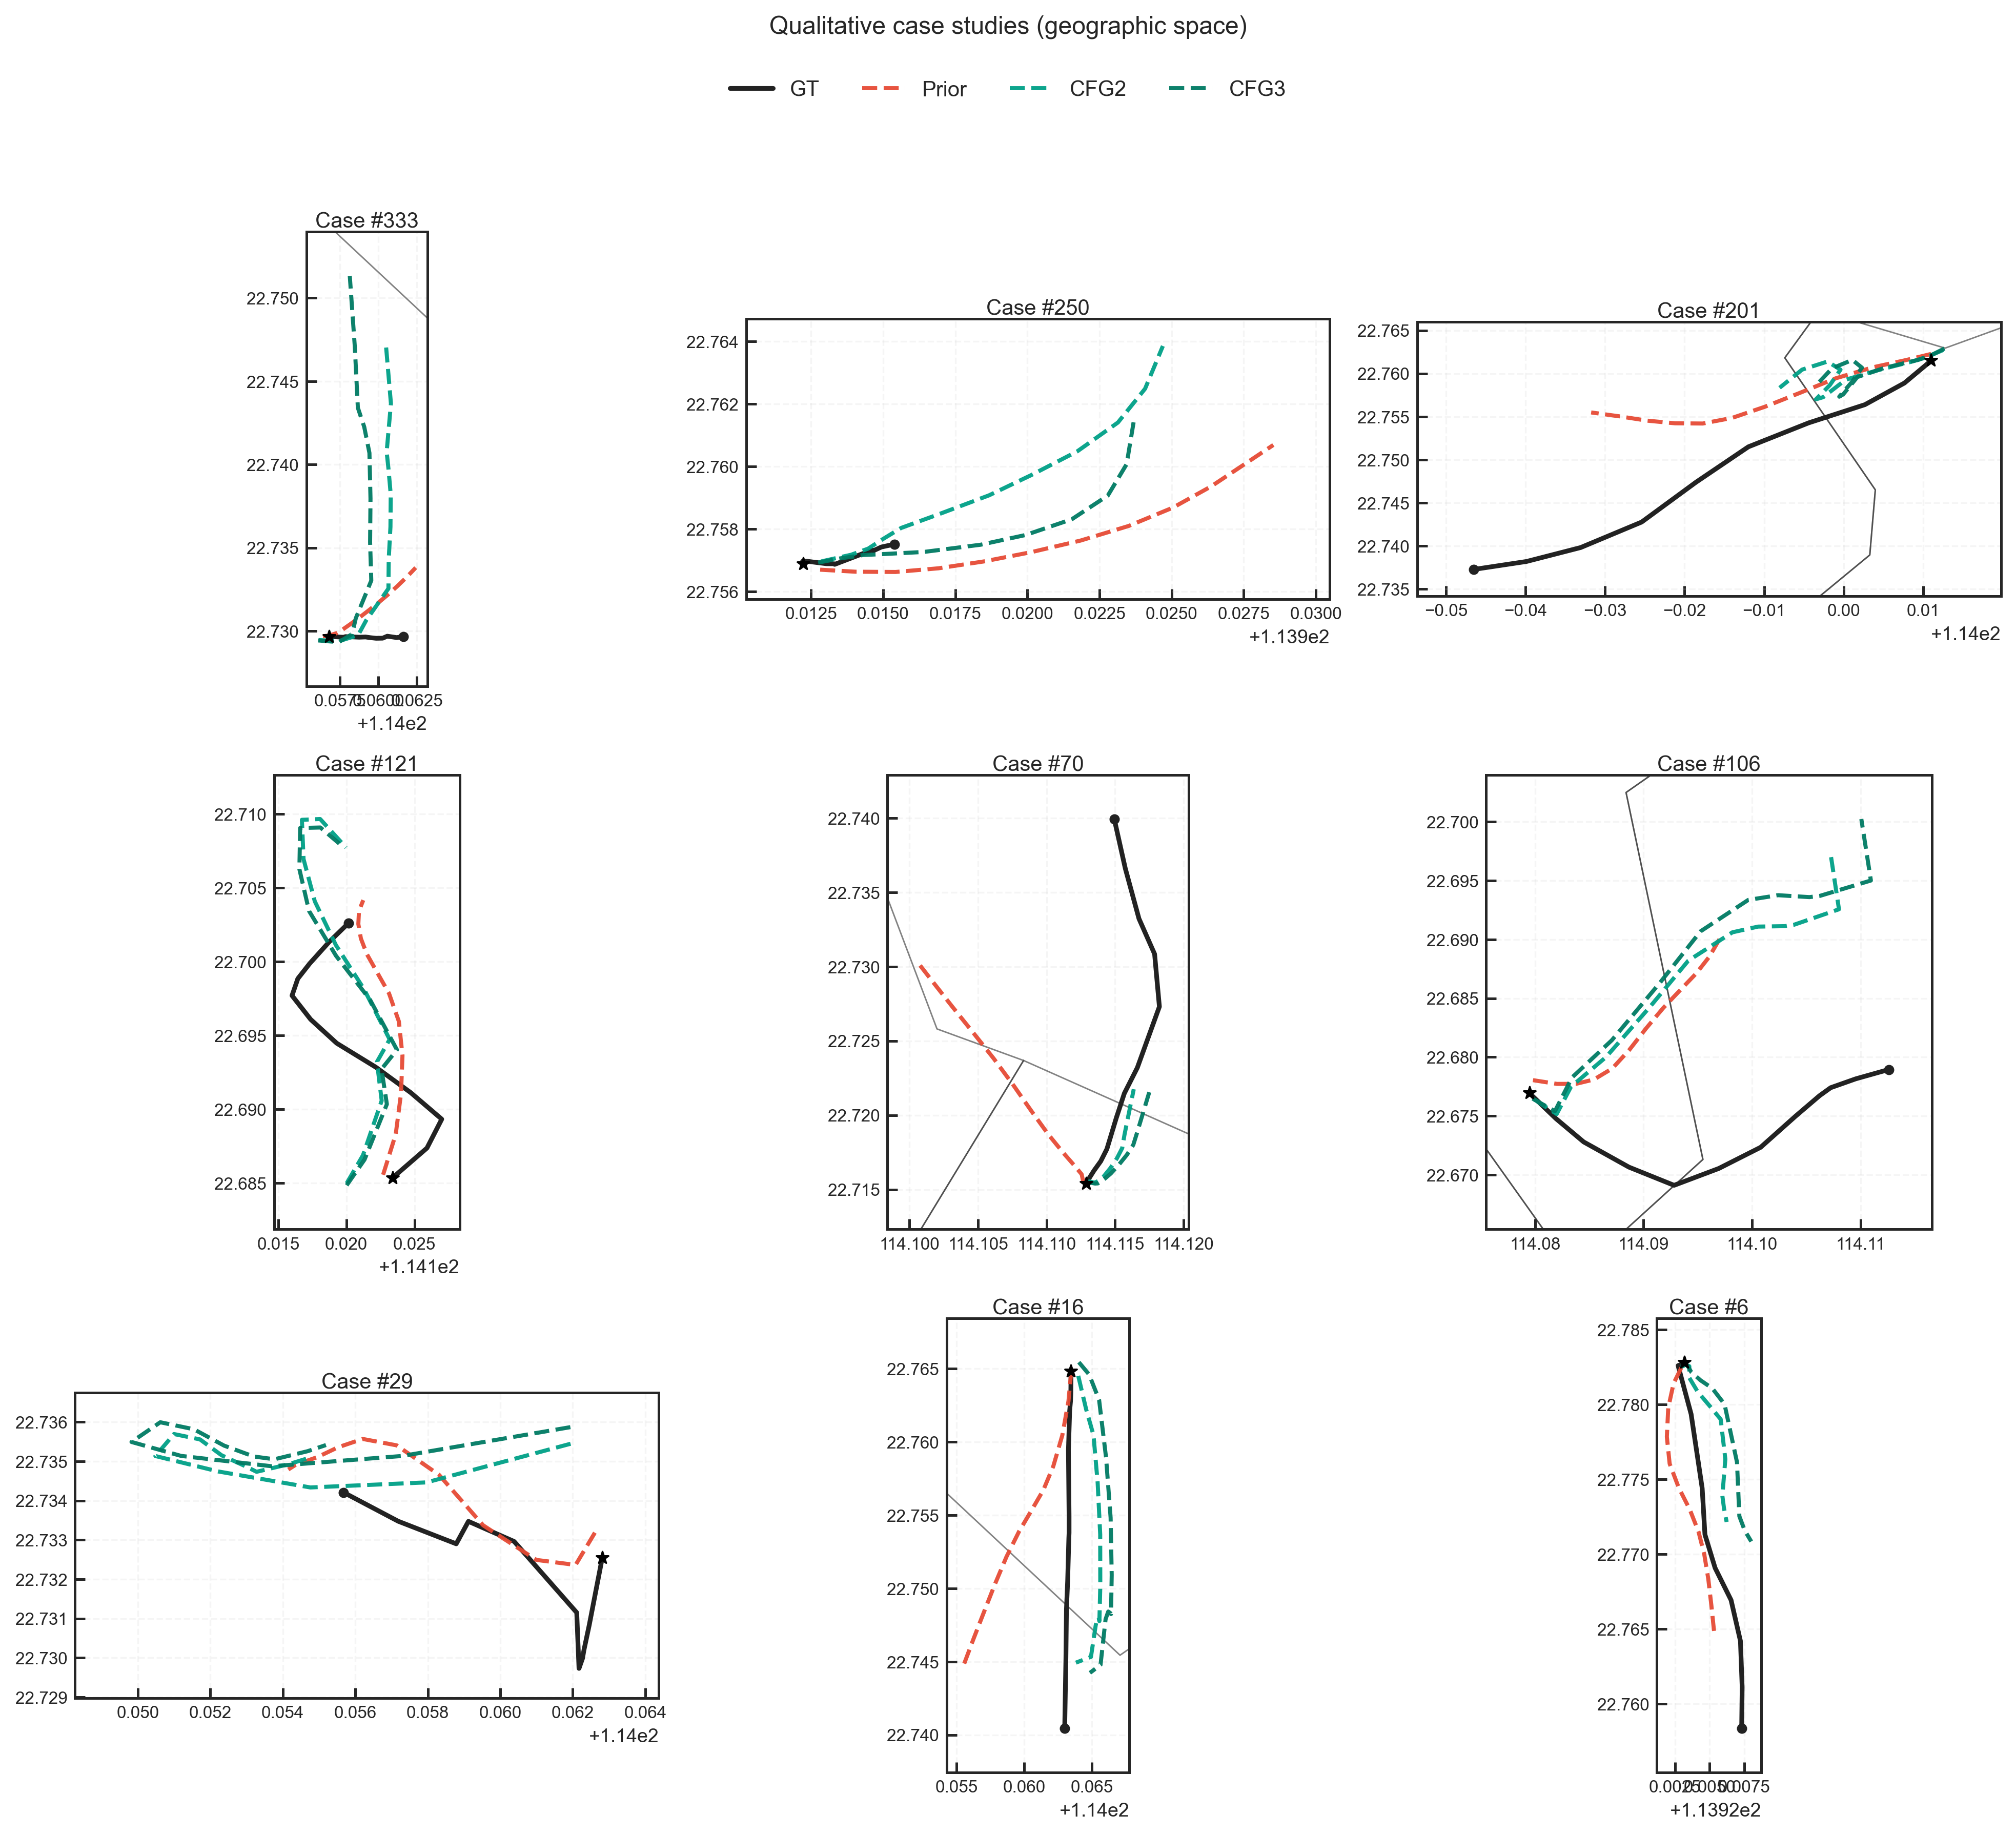
\includegraphics[width=0.98\linewidth]{figures/stage_cfg/fig_geo_case_study_cfg.png}
  \caption{Micro-scale qualitative case studies in geographic space: for the same OD condition, we compare GT, deterministic prior, and two CFG settings (cfg=2/3). Each subplot uses a local zoom extent to highlight route-shape differences.}
  \label{fig:cfg_case_study}
\end{figure}
